\documentclass{amsart}
\usepackage[utf8]{inputenc}
\usepackage{accents}
\usepackage{graphicx}
\usepackage{amsfonts}
\usepackage{listings}
\usepackage{amscd}
\usepackage{amssymb}
\usepackage{hyperref}
\usepackage{url}
\usepackage{tikz}
\usepackage[a4paper,margin=1in]{geometry}
\newtheorem{theorem}{Theorem}
\newtheorem{lemma}[theorem]{Lemma}
\newtheorem{corollary}[theorem]{Corollary}
\newtheorem{proposition}[theorem]{Proposition}
\theoremstyle{definition}
\newtheorem{definition}[theorem]{Definition}
\newtheorem{example}[theorem]{Example}
\theoremstyle{remark}
\newtheorem{remark}[theorem]{Remark}
\newcommand{\abs}[1]{\lvert#1\rvert}
\newcommand{\ZZ}{\mathbb Z}
\newcommand{\QQ}{\mathbb Q}
\newcommand{\RR}{\mathbb R}
\newcommand{\NN}{\mathbb N}
\newcommand{\CC}{\mathbb C}
\newcommand{\From}{\colon}
\newcommand{\To}{\rightarrow}

\lstset{
language=R,
basicstyle=\scriptsize\ttfamily,
commentstyle=\ttfamily\color{gray},
numbers=left,
numberstyle=\ttfamily\color{gray}\footnotesize,
stepnumber=1,
numbersep=5pt,
backgroundcolor=\color{white},
showspaces=false,
showstringspaces=false,
showtabs=false,
frame=single,
tabsize=2,
captionpos=b,
breaklines=true,
breakatwhitespace=false,
title=\lstname,
escapeinside={},
keywordstyle={},
morekeywords={},
numbers=none
}


%---------EDIT THE CONTENTS TITLE/AUTHOR INFO BELOW!
\title{YSC4204: Statistical Computing\\
Problem Set 2}
\author{East: Sean Saito, John Reid, Hrishi Olickel, Chong Woon Han}
\date{\today}

%-----------THIS IS WHERE THE GOOD STUFF BEGINS.
\begin{document}

\maketitle

\begin{enumerate}
%1
\item
The C code to implement meanC() is as follows:
\begin{lstlisting}[language=C]
#include <stdio.h>
#include <R.h>

/*
* Function that calculates the mean of vector x
* Inputs:
*     x   : vector of doubles
*     n   : length of vector
*     res : placeholder for result
*/
void meanC(double *x, int *n, double *res) {

  int i;
  double temp = 0.0;
  for (i = 0; i < *n; i++) {
    temp += x[i];
  }

  *res = temp / *n;
  return;
}
\end{lstlisting}
We call this function in R using the following R Code:
\begin{lstlisting}[language=R]
# Automatically sets working directory to source file location
this.dir <- dirname(parent.frame(2)$ofile)
setwd(this.dir)

# Problem 1 - Writing a mean function in C to be used in R
meanR <- function(x) {
  # Placeholder for result
  res = 0.0
  n = length(x)
  
  dyn.load("mean.so")
  m = .C("meanC", x=as.double(x), n=n, res=res)
  
  return(m$res)
}
\end{lstlisting}
%2
\item
\begin{enumerate}
%a
\item OMG

%b
\item y is dis so hard?

\end{enumerate}
%3
\item
Question 3 here
%4
\item
Suppose $x \sim$ Rayleigh($\sigma$). The Rayleigh probability density function is
$$ f(x) = \frac{x}{\sigma^2}e^{-x^2/(2\sigma^2)}, \hspace{0.5cm} x \geq 0, \sigma >0.$$
The cumulative distribution function is
$$ F(x) = 1 - e^{-x^2/(2\sigma^2)} \text{ for } x \in [0,\infty).$$
We derive $F^{-1}_X(x)$ as follows:
\begin{align*}
y &= 1 - e^{-x^2/(2\sigma^2)},\\
e^{-x^2/(2\sigma^2)} &= 1-y,\\
\frac{-x^2}{2\sigma^2} &= \ln (1-y),\\
x &= \sqrt{-2\sigma^2 \ln (1-y)},\\
F^{-1}_X(x) &= \sqrt{-2\sigma^2 \ln (1-y)}.
\end{align*}
For $u \sim$ Uniform$(0,1)$, and given that $U$ and $1-U$ have the same distribution, we can generate Rayleigh random variables by taking
$$ F^{-1}_X(u) = \sqrt{-2\sigma^2 \ln (u)}.$$
We implement this equation in R to generate $n$ random samples from a Rayleigh($\sigma$) distribution as shown below:
\begin{lstlisting}[language=R]
## Define function to generate Rayleigh random variables ##
rray <- function(n,sigma){
  u <- runif(n)
  output <- sqrt(-2*sigma^2*log(u))
  return(output)
}
\end{lstlisting}
The code used to generate histograms is as follows:
\begin{lstlisting}[language=R]
## Set seed to ensure consistency before generating numbers and plotting ##
set.seed(0)

########## simga = 0.5 ##########
x1 <- rray(10000,0.5)
hist(x1,prob=TRUE,
     main="Generated rayleigh random variables with sigma=0.5",
     xlab="x") # plot the histogram

## Superimpose a density line ##
xlines1 <- seq(0,round(max(x1)),0.01)
ylines1 <- (xlines1/0.5^2)*exp(-xlines1^2/(2*(0.5^2)))
lines(xlines1,ylines1)

########## sigma = 2 ##########
x2 <- rray(10000,2)
hist(x2,prob=TRUE,
     main="Generated rayleigh random variables with sigma=2",
     xlab="x") # plot the histogram

## Superimpose a density line ##
xlines2 <- seq(0,round(max(x2)),0.01)
ylines2 <- (xlines2/2^2)*exp(-xlines2^2/(2*(2^2)))
lines(xlines2,ylines2)
\end{lstlisting}
The resulting histograms are show below:\\
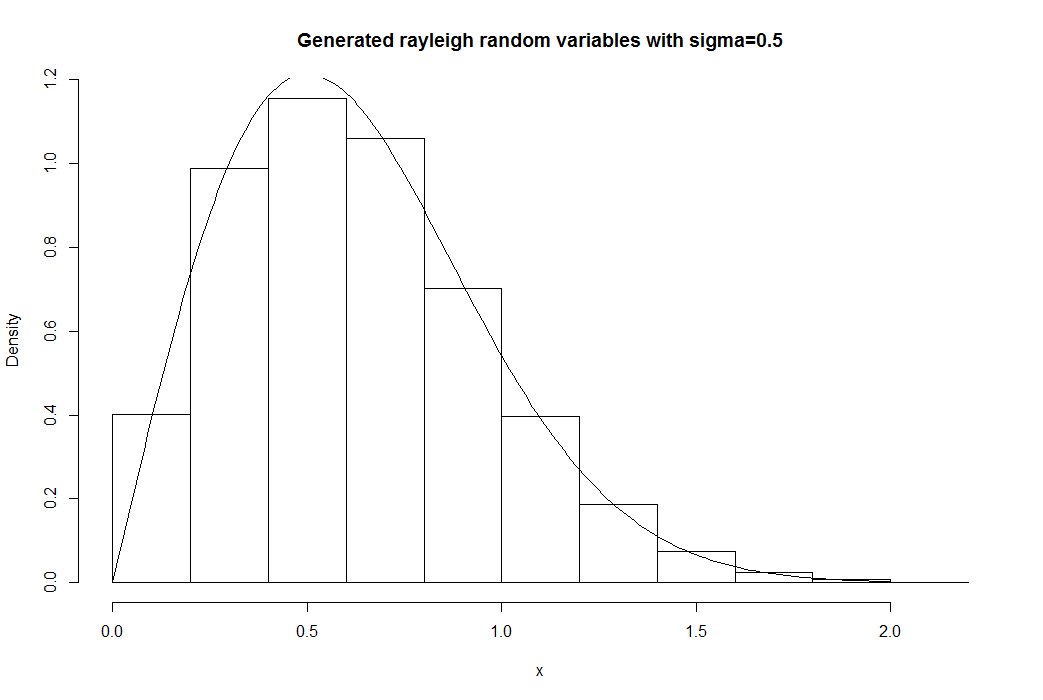
\includegraphics[scale=0.6]{rayleigh_0_5}
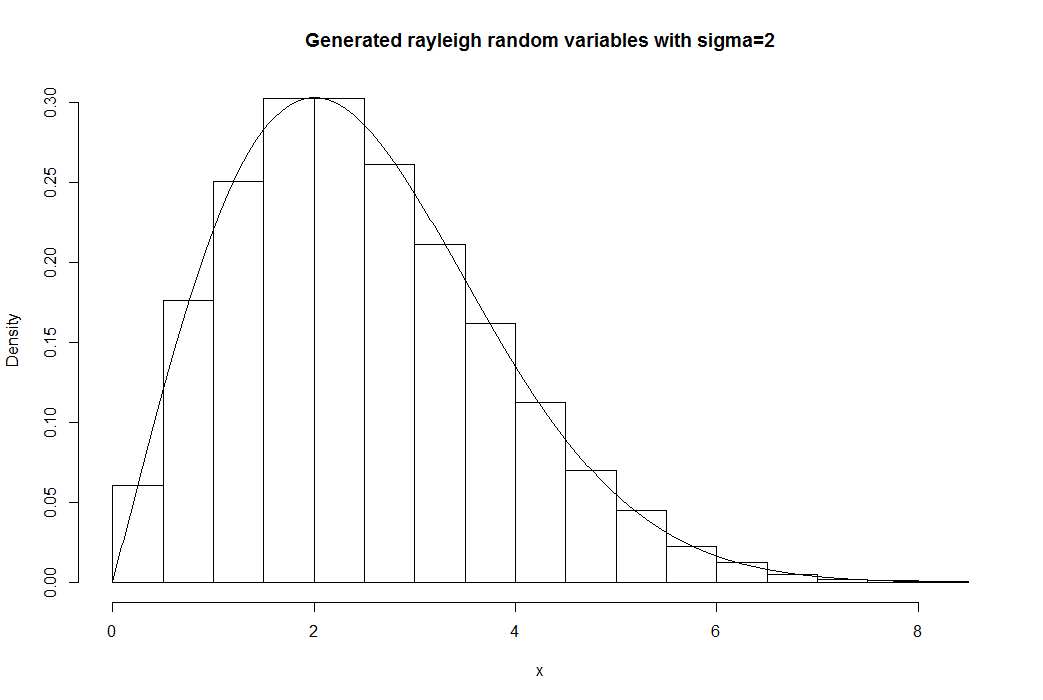
\includegraphics[scale=0.6]{rayleigh_2}
\end{enumerate}
\end{document}